\documentclass[problem]{mcs}

\begin{pcomments}
  \pcomment{CP_the_four_door_deal}
  \pcomment{from: S09.cp12r -- commented out}
\end{pcomments}

\pkeywords{
  probability
}

%%%%%%%%%%%%%%%%%%%%%%%%%%%%%%%%%%%%%%%%%%%%%%%%%%%%%%%%%%%%%%%%%%%%%
% Problem starts here
%%%%%%%%%%%%%%%%%%%%%%%%%%%%%%%%%%%%%%%%%%%%%%%%%%%%%%%%%%%%%%%%%%%%%

% S09

\begin{problem}
\textbf{[The Four-Door Deal]}
Suppose that {\em Let's Make a Deal} is played according to different
rules.  Now there are \textbf{four} doors, with a prize hidden
behind one of them.  The contestant is allowed to pick a door.  The
host must then reveal a different door that has no prize behind it.
The contestant is allowed to stay with his or her original door or to
pick one of the other two that are still closed.  If the contestant
chooses the door concealing the prize in this second stage, then he or
she wins.

\bparts

\ppart Contestant Stu, a sanitation engineer from Trenton, New Jersey,
stays with his original door.  What is the probability that he wins
the prize?

The tree diagram is awkwardly large.  This often happens; in fact,
sometimes you'll encounter \textit{infinite} tree diagrams!  Try to
draw enough of the diagram so that you understand the structure of the
remainder.

\begin{solution}
Let's make the same assumptions as in the original
problem:
%
\begin{enumerate}
\item The prize is equally likely to be behind each door.
\item The contestant is equally likely to pick each door initially,
regardless of the prize's location.
\item The host is equally likely to reveal each door that does not
conceal the prize and was not selected by the player.
\end{enumerate}
%
A partial tree diagram is shown below.  The remaining subtrees are
symmetric to the fully-expanded subtree.
%
\begin{center}
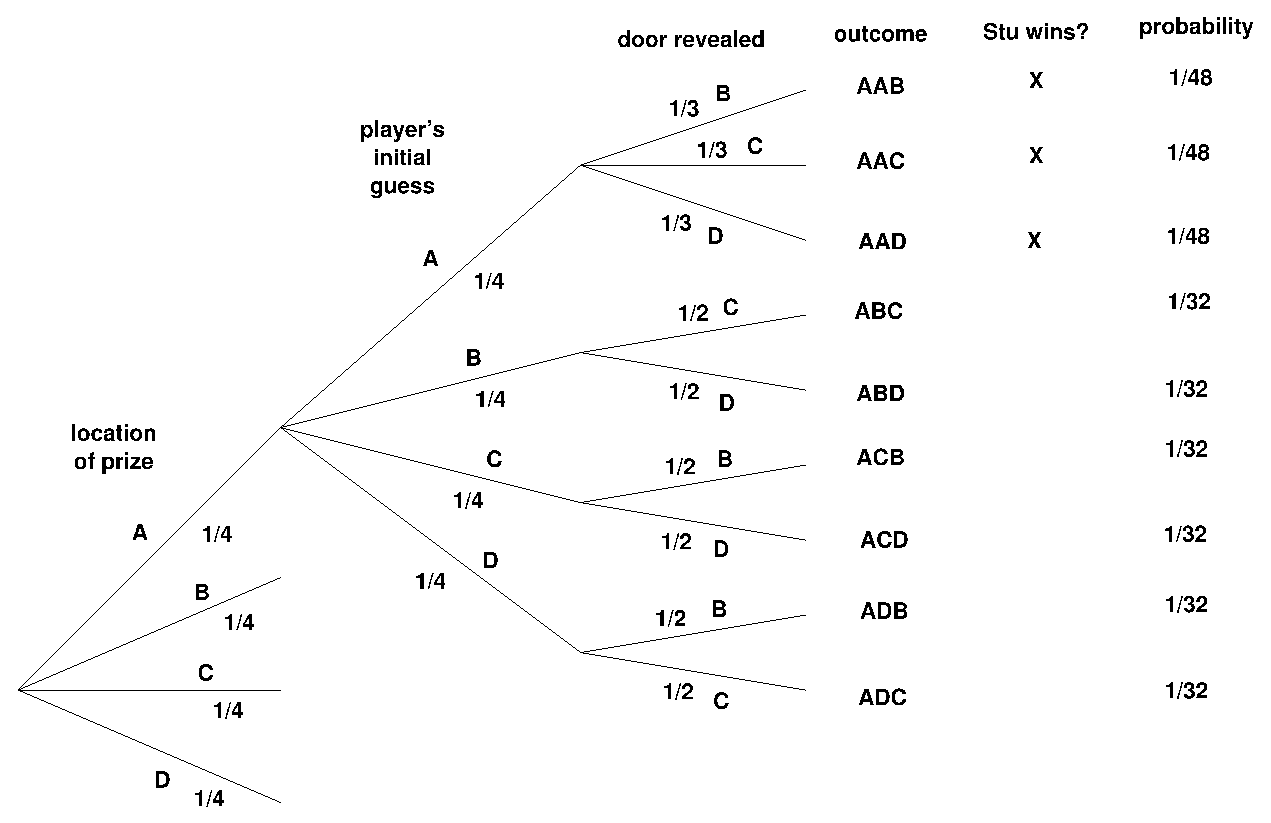
\includegraphics[width=6in]{figures/four-door}
\end{center}
%
The probability that Stu wins the prize is:
%
\[
\pr{\text{Stu wins}} = 4 \cdot \left(\frac{1}{48} + \frac{1}{48} + \frac{1}{48}\right) = \frac{1}{4}
\]
%
We multiply by 4 to account for the four subtrees, of which we've only
drawn one.

Notice that we expanded the tree out to the third (``door revealed'')
level to spell out the outcomes, but in this case we could, in fact, have
stopped at the second level (``player's initial guess'').  This follows
because the win/lose outcome is determined by the prize location and Stu's
selected door, regardless of what happens after that.
\end{solution}

\ppart Contestant Zelda, an alien abduction researcher from Helena,
Montana, switches to one of the remaining two doors with equal
probability.  What is the probability that she wins the prize?

\begin{solution}
A partial tree diagram is worked out below.
%
\begin{center}
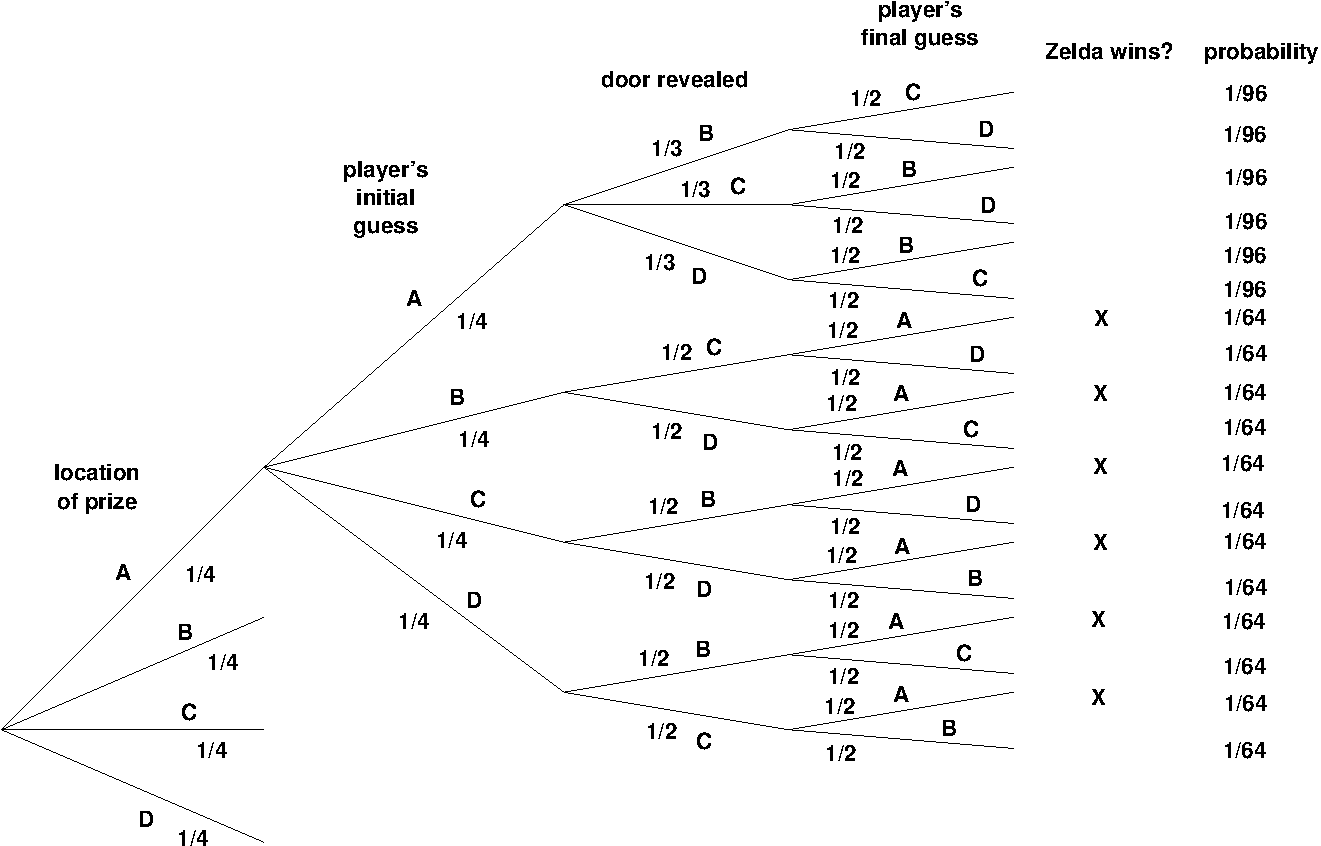
\includegraphics[width=6in]{figures/four-doorb}
\end{center}
%
The probability that Zelda wins the prize is:
%
\[
\pr{\text{Zelda wins}} = 4 \cdot \left( \frac{1}{64} + \frac{1}{64} + \frac{1}{64} + \frac{1}{64} + \frac{1}{64} + \frac{1}{64} \right) = \frac{3}{8}
\]
\end{solution}
\eparts

\end{problem}


%%%%%%%%%%%%%%%%%%%%%%%%%%%%%%%%%%%%%%%%%%%%%%%%%%%%%%%%%%%%%%%%%%%%%
% Problem ends here
%%%%%%%%%%%%%%%%%%%%%%%%%%%%%%%%%%%%%%%%%%%%%%%%%%%%%%%%%%%%%%%%%%%%%

\endinput